\documentclass{article}

\usepackage{graphicx} % for EPS, load graphicx instead
% set up tight list spacing
\usepackage{enumitem} 
\setlist{nolistsep,nosep}

% for toggles
\usepackage{etoolbox}

\newcommand {\studyquote}[1]{\em ``#1''\normalfont}

% CHANGE FROM TOGGLE TRUE TO TOGGLE FALSE FOR NON-ANONYMOUS RENDERING
% http://tex.stackexchange.com/questions/5894/latex-conditional-expression
\newtoggle{anonymous}
\togglefalse{anonymous}
%\togglefalse{anonymous}

% CHANGE FROM TOGGLE TRUE TO TOGGLE FALSE TO HIDE COMMENTS
\newtoggle{comments}
\toggletrue{comments}
%\togglefalse{comments}

% Comment region command (from Wesley Willett)
\usepackage[usenames]{color}
\usepackage[usenames,dvipsnames]{xcolor}
\iftoggle{comments} {
  %if we want to show comments
  \newcommand {\ben}[1]{{\color{violet}\bf{BZ: #1}\normalfont}}
  \newcommand {\ai}[1]{{\color{BrickRed}\bf{BH: #1}\normalfont}}
}{
  %if we don't want to show comments
  \newcommand {\ben}[1]{}
  \newcommand {\ai}[1]{}
}

%%% Local Variables: 
%%% mode: latex
%%% TeX-master: "report"
%%% End: 



\begin{document}

\title{Model OpenWSN (TSCH) protocol A Ptolemy Approach}

\iftoggle{anonymous}{
\author{
 \alignauthor Anonymous for submission\\
    %\affaddr{...}\\
    %\email{...}\\
  }
}{ %else
  \author{
  Antonio Iannopollo, Ben Zhang\\
  EECS, UC Berkeley\\
  \{antonio, benzh\}@eecs.berkeley.edu \\
}

}

\maketitle

\begin{abstract}
\end{abstract}


%% refer to http://www.acm.org/about/class/ccs98-html
% \category{H.5.2.}{Information Interfaces and Presentation (e.g. HCI)}{Interaction styles (e.g., commands, menus, forms, direct manipulation)}.
% \vfill\eject

\section{Introduction}
We want to model the OpenWSN \cite{watteyne2012openwsn} stack using Ptolemy II \cite{davis1999overview}. Our goal is to provide a tool to estimate power consumption, scalability and network behavior of a WSN application in an early phase of the design process.

Once completed, this project will provide a two-fold contribution. First, it is going to augment the building blocks available to the Ptolemy community. This means Ptolemy will be used to design applications with a clear high level semantics, while being able to evaluate lower level details and their impact once the application is deployed. Second, we are providing a tool to help the OpenWSN community in the development process.

We are focusing on modeling the MAC layer of OpenWSN. This layer implements the IEEE 802.15.4e protocol standard, based on a time synchronized channel hopping technique. We decided to model this stack layer because each state of the protocol state machine is associated with a single state of the radio. Modeling power consumption dynamics is, in this way, straightforward (we refer to \cite{vilajosana2013realistic} for details). Moreover, at this level it is possible to capture point to point communication issues and the impact of a network schedule, required by 802.15.4e. 

%%% Local Variables: 
%%% mode: latex
%%% TeX-master: "report"
%%% End: 

\section{Project Status}
\label{sec:project-status}

\subsection{Modeling Clock Drift}
\label{sec:modeling-clock-drift}
In previous implementations, we modeled clocks generating an event for each clock tick. Modeling drift was achieved by changing the rate of clock event generation for each node.
In the actual implementation we don't have an event for each clock tick, and drift is modeled using the Ptolemy support for multiform time. Figure \ref{fig:time} shows clock drift for one node, compared to the global model clock.

\begin{figure}
  \centering
  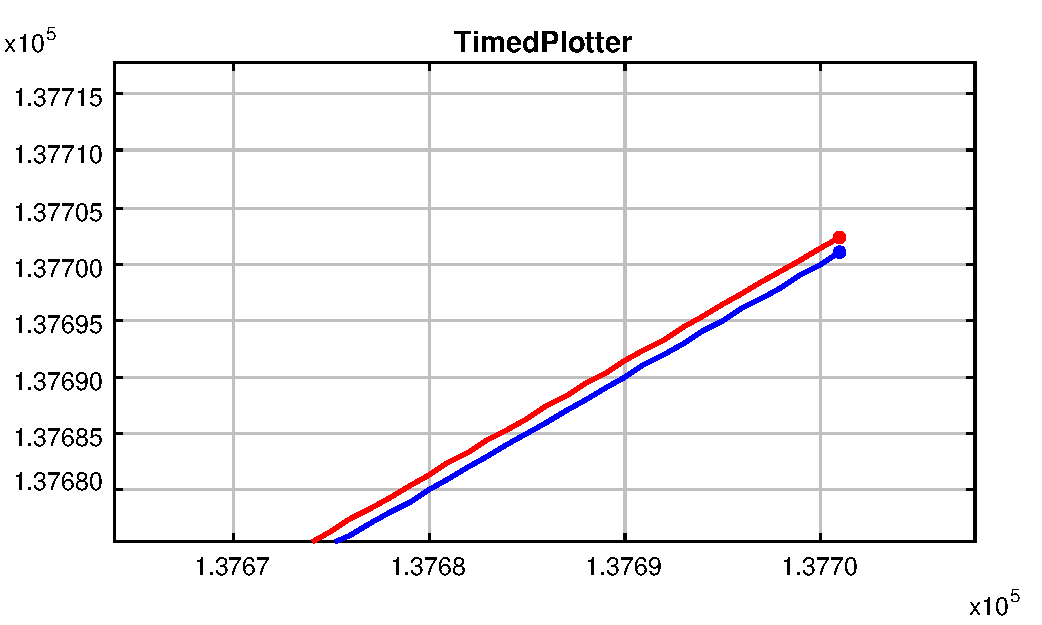
\includegraphics[width=\textwidth]{figures/time-drift.pdf}
  \caption{Clock drift modeling in Ptolemy using Multiform time}
  \label{fig:time}
\end{figure}

\subsection{Modeling the IEEE 802.15.4e state machine}
\label{sec:modeling-state-machine}

We modeled the IEEE 802.15.4e finite state machine using Ptolemy modal modes. The result is the hierarchical FSM shown in figure \ref{fig:fsm}. Figure \ref{fig:tx} shows the refinement of the \emph{transmission} state of the high level FSM. All other states of the high level FSM (\emph{reception}, \emph{SLEEP} and \emph{synchronization}) are similarly refined.

\begin{figure}
  \centering
  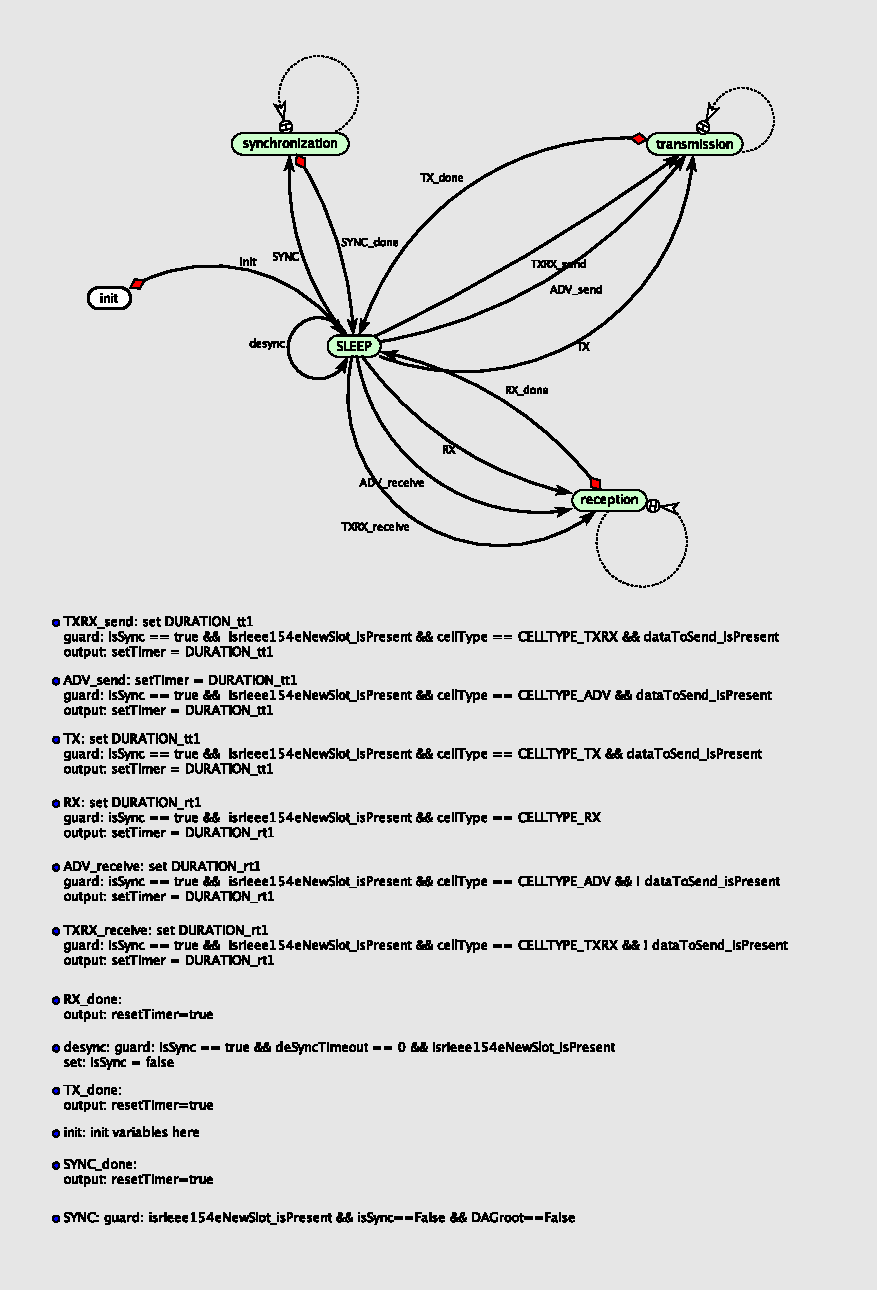
\includegraphics[width=\textwidth]{figures/FSM.pdf}
  \caption{High level FSM of the IEEE 802.15.4e protocol standard}
  \label{fig:fsm}
\end{figure}

\begin{figure}
  \centering
  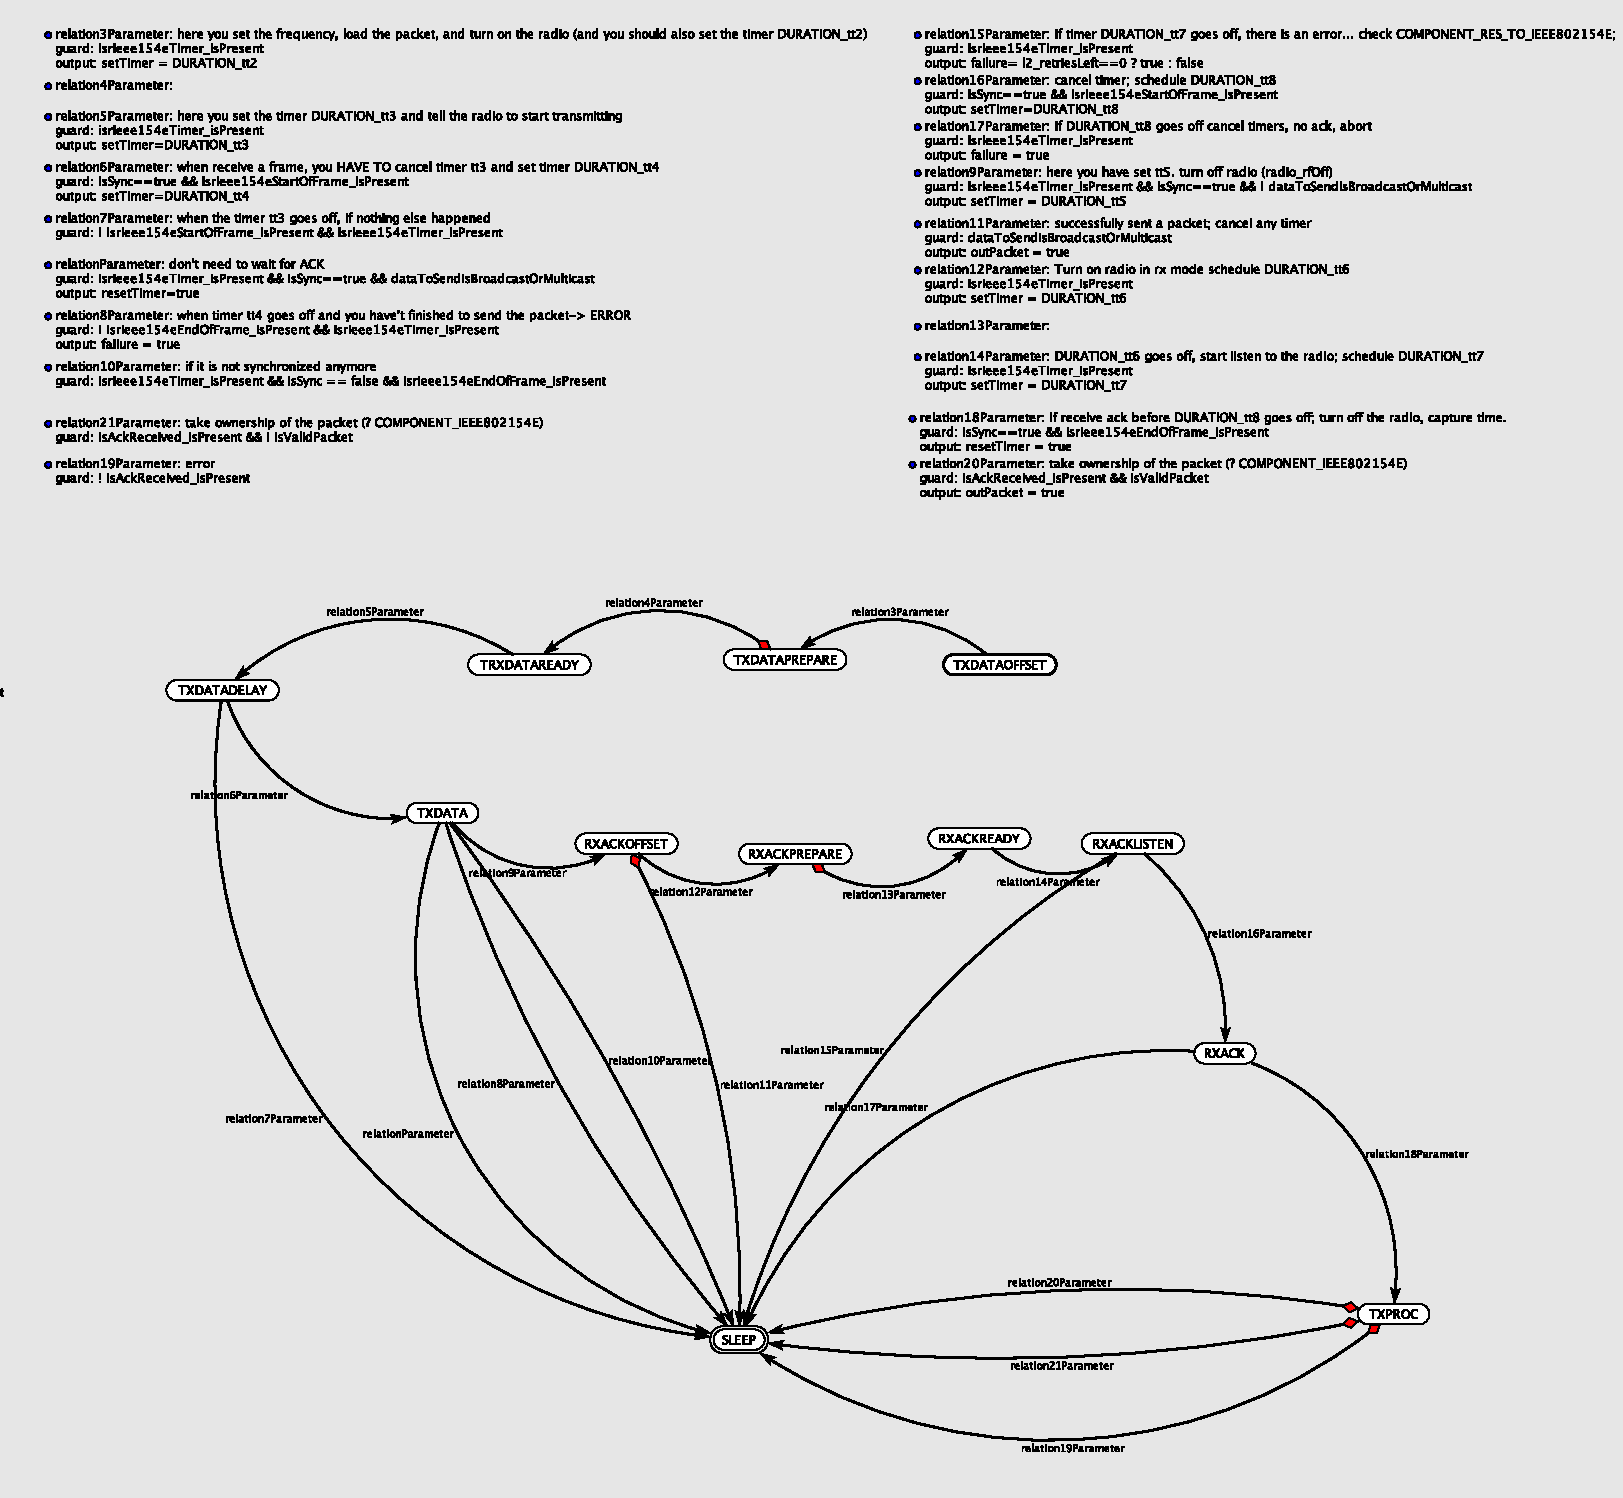
\includegraphics[width=\textwidth]{figures/TransmissionFSM.pdf}
  \caption{Transmission state refinement}
  \label{fig:tx}
\end{figure}

\subsection{Modeling the Physical Layer}
\label{sec:modeling-physical-layer}
Physical layer is modeled as a discrete event model. The physical layer is used to communicate with the MAC layer information such us the beginning and the end of the reception of a packet. Figure \ref{fig:node} shows the actual structure of a node model (a DE model), including the relation between the physical and the MAC layers.

\begin{figure}
  \centering
  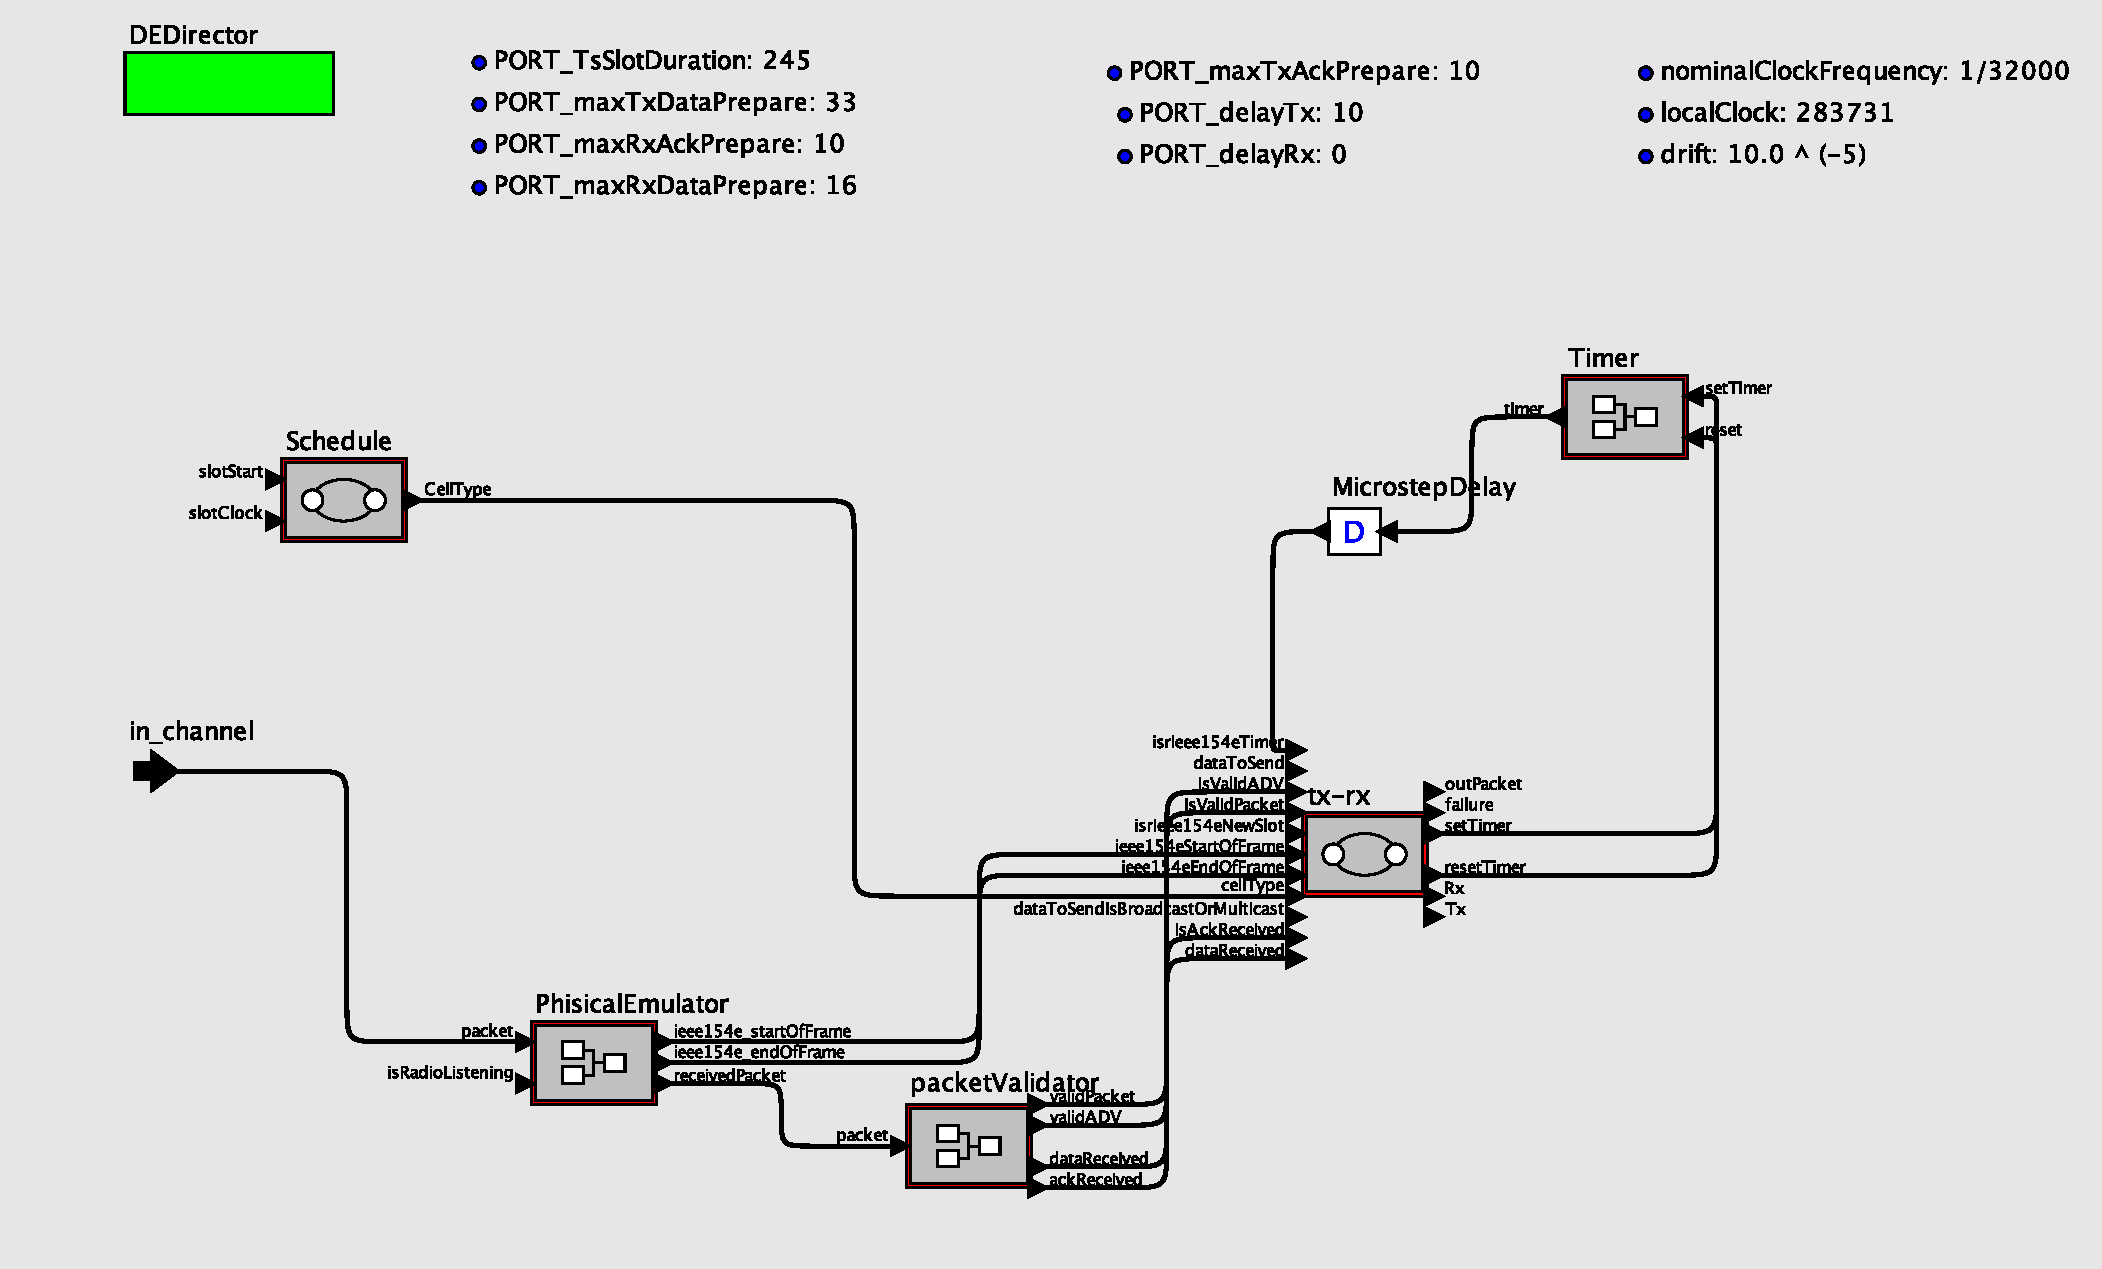
\includegraphics[width=\textwidth]{figures/WirelessNode.pdf}
  \caption{Interaction between different actors composing a node}
  \label{fig:node}
\end{figure}


\subsection{Modeling the scheduler}
\label{sec:modeling-scheduler}
In our model, the scheduler is represented as a FSM. At this point, we don't support a dynamic scheduler. In particular, our implementation of the scheduler reflects the OpenWSN implementation, where the scheduler is hard-coded in the MAC layer. Figure \ref{fig:scheduler} shows our implementation of the scheduler. Unconnected states represent other available scheduler slot types, not used in the OpenWSN implementation. Implementing a dynamic scheduler is a goal of future work.

\begin{figure}
  \centering
  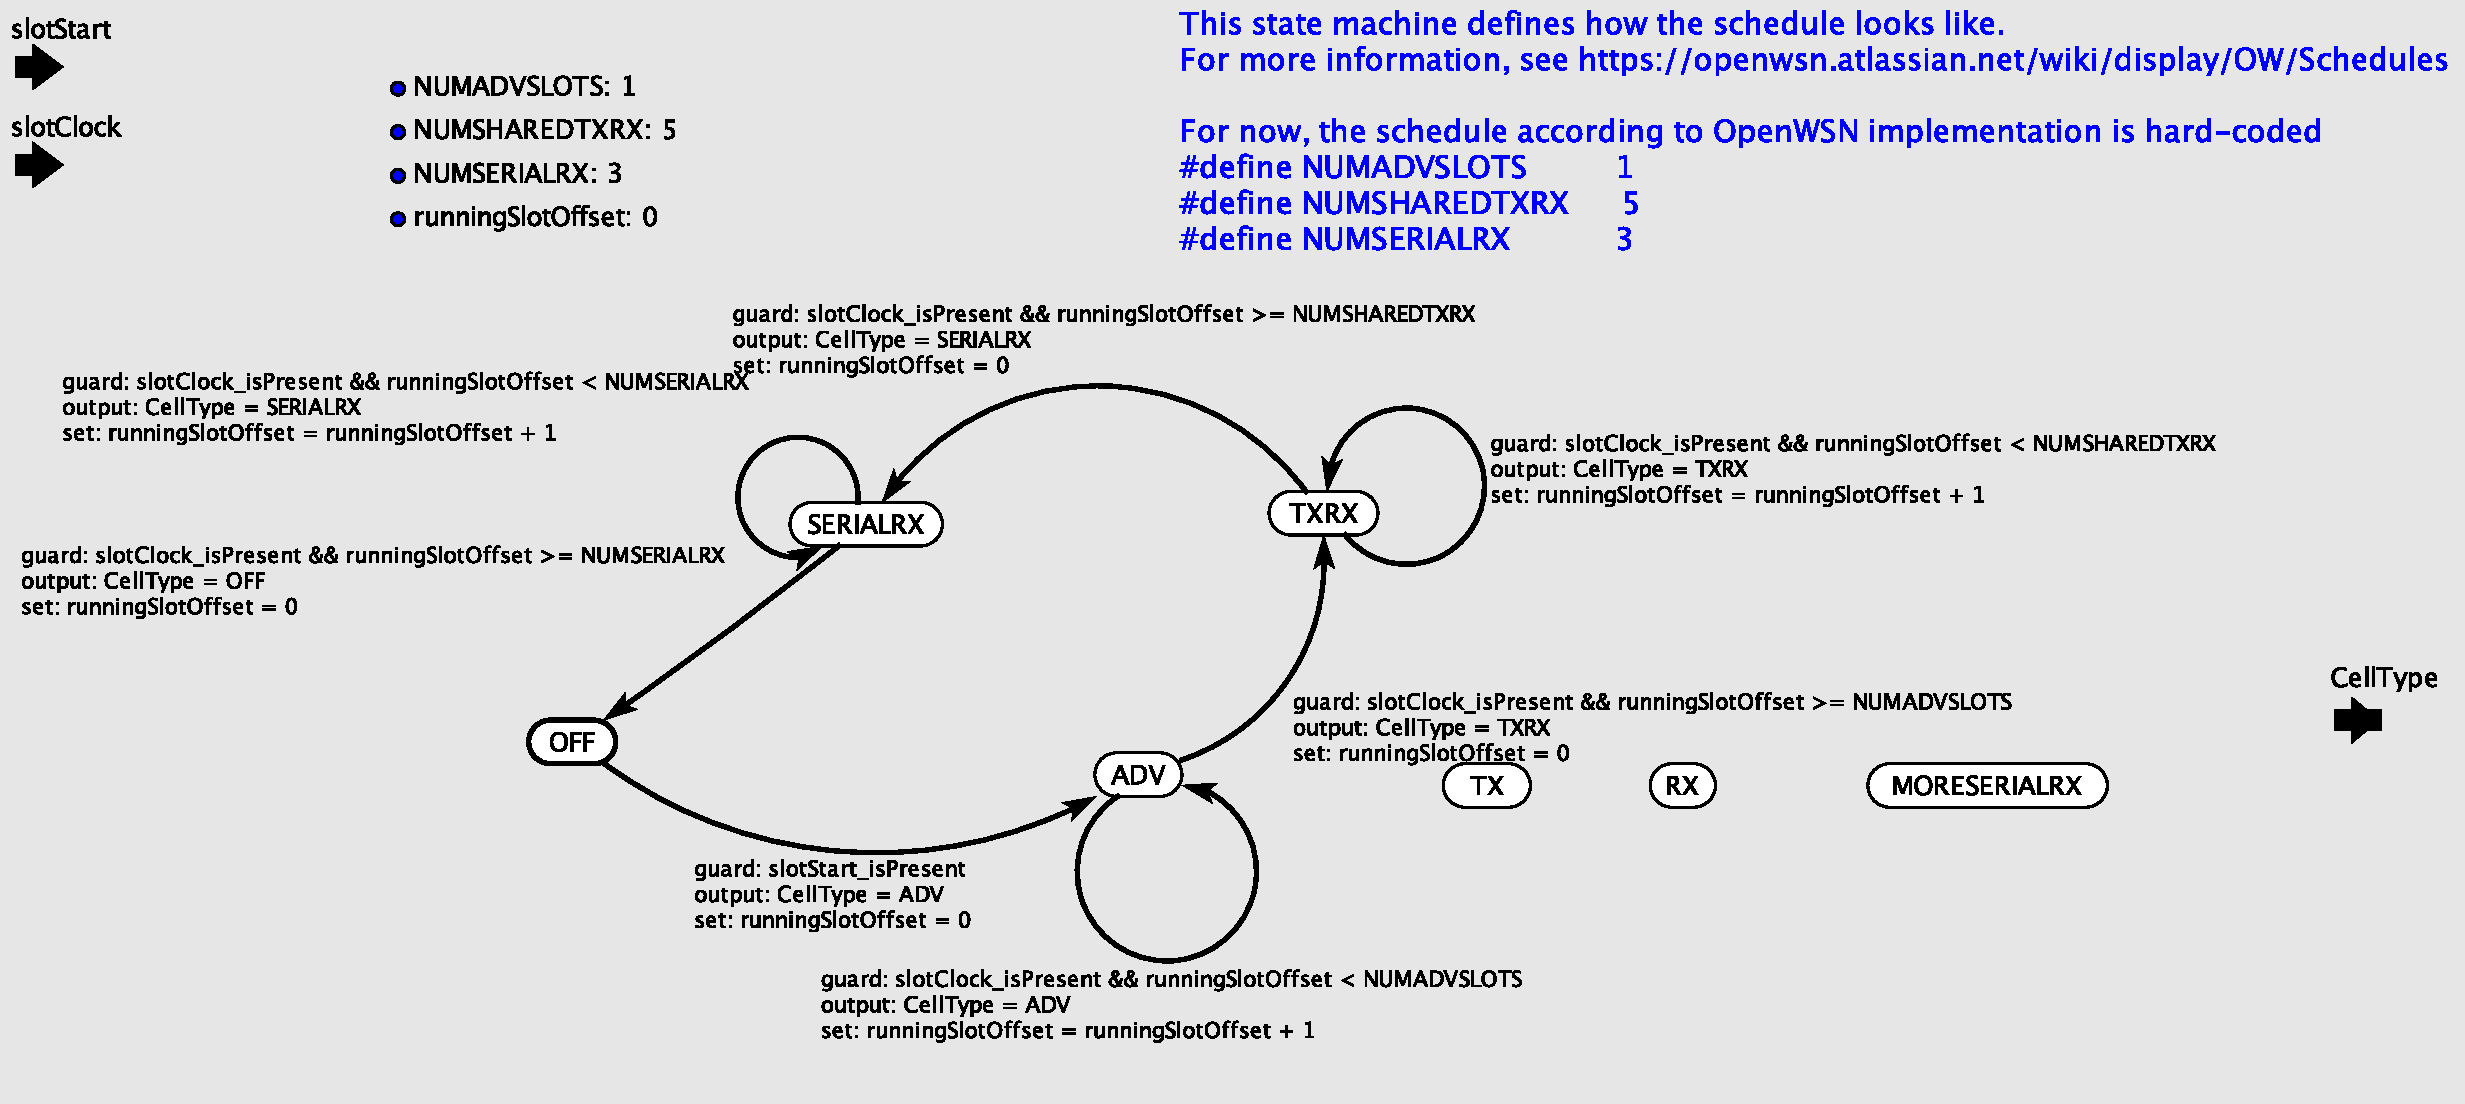
\includegraphics[width=\textwidth]{figures/Scheduler.pdf}
  \caption{Scheduler FSM}
  \label{fig:scheduler}
\end{figure}

%%% Local Variables: 
%%% mode: latex
%%% TeX-master: "report"
%%% End: 


\section{Conclusion}
\label{sec:conclusion}

Work is proceeding smoothly following our previous roadmap (with minor changes). We are extending our model according to an iterative approach, which allows us to capture feedback and fix issues while improving its functionality. By the end of the month, we plan to simulate inter-node communication and time synchronization, tag each execution with a specific power consumption index.



%%% Local Variables: 
%%% mode: latex
%%% TeX-master: "report"
%%% End: 


%figure template:
%\begin{figure}[!h]
%\centering
%\includegraphics[width=1.0\columnwidth]{Figure1}
%\caption{With Caption Below, be sure to have a good resolution image
%  (see item D within the preparation instructions).}
%\label{fig:figure1}
%\end{figure}

% Balancing columns in a ref list is a bit of a pain because you
% either use a hack like flushend or balance, or manually insert
% a column break.  http://www.tex.ac.uk/cgi-bin/texfaq2html?label=balance
% multicols doesn't work because we're already in two-column mode,
% and flushend isn't awesome, so I choose balance.  See this
% for more info: http://cs.brown.edu/system/software/latex/doc/balance.pdf
%
% Note that in a perfect world balance wants to be in the first
% column of the last page.
%
% If balance doesn't work for you, you can remove that and
% hard-code a column break into the bbl file right before you
% submit:
%
% http://stackoverflow.com/questions/2149854/how-to-manually-equalize-columns-
% in-an-ieee-paper-if-using-bibtex
%
% Or, just remove \balance and give up on balancing the last page.
%
%% \balance

\bibliographystyle{acm-sigchi}
\bibliography{uist14}
\end{document}
